\apendice{Plan de proyecto software}

\section{Introducción}
Antes de empezar los proyectos, es clave tener en cuenta el tiempo, costos etc. Planificar bien evita problemas más adelante, permite usar el tiempo y los recursos de manera efectiva, y asegura que el proyecto sea legalmente viable.

\section{Planificación temporal}
En la aplicación de GitHub se propusieron varias tareas (issues), estas se agrupan en milestones cuando están relacionadas entre ellas. 

Desglose del proyecto por cada tarea y los diferentes subojetivos que se vuscaban al realizarla:

\begin{enumerate}
    \item Investigación y planificación
    \begin{itemize}
        \item Definir objetivos y comprender los requisitos del proyecto.
        \item Investigación sobre métodos de conexión de hardware.
        \item Plan de trabajo detallado.
        \item Selección de componentes hardware adecuados.
        \item Estudio de algoritmos de predicción.
    \end{itemize}

    \item Montaje del sensor con arduino y pruebas de conexión
    \begin{itemize}
        \item Montaje del hardware del sensor AD8232.
        \item Configuración inicial del software para la lectura de datos.
        \item Pruebas del correcto funcionamiento del dispositivo.
        \item Evaluación y selección del método de conexión óptimo.
    \end{itemize}

    \item Diseño de la ventana de datos en vivo (\textit{serialmonitor.py})
\begin{itemize}
    \item Funcionalidades de la ventana de datos en vivo:
        \begin{itemize}
            \item Visualizar datos en tiempo real.
            \item Seleccionar el puerto COM.
            \item Grabar los datos de ECG.
        \end{itemize}
\end{itemize}


    \item Modelo de Predicción de los tipos de ciclo cardíaco
    \begin{itemize}
        \item Estudio del modelo de predicción mas óptimo.
        \item Implementación de un modelo de predicción basado en Random Forest.
        \item Entrenamiento y evaluación del modelo con datos de ECG.
        \item Ajustes y optimización del modelo para mejorar la precisión.
    \end{itemize}

    \item Desarrollo de la aplicación web
    \begin{itemize}
        \item Implementación del backend para la recepción y procesamiento de datos.
        \item Desarrollo del frontend para la visualización de datos y resultados.
        \item Funciones para cargar y analizar archivos de datos con el modelo de predicción entrenado.
        \item Implementación de la funcionalidad de guardado de predicciones en la base de datos.
    \end{itemize}

    \item Mejoras (base de datos y calidad de datos) y pruebas finales
    \begin{itemize}
        \item Optimización de la base de datos para un acceso más eficiente.
        \item Implementación de mejoras en la calidad de los datos recolectados.
        \item Pruebas exhaustivas del sistema completo.
        \item Ajustes finales basados en los resultados de las pruebas.
    \end{itemize}

    \item Redacción de la Memoria
    \begin{itemize}
        \item Resumen y abstract
        \item Introducción
        \item Objetivos
        \item Conceptos teóricos
        \item Metodología
        \item Resultados
        \item Conclusiones
        \item Bibliografía
    \end{itemize}

    \item Redacción de Anexos
    \begin{itemize}
        \item A. Plan de proyecto software
        \item B. Documentacion de usuario
        \item C. Manual de desarrollador / programador / investigador
        \item D. Descripción de adquisición y tratamiento de datos
        \item E. Manual de especificación de diseño
        \item F. Especificación de requisitos
        \item G. Estudio experimental
        \item H. Anexo de sostenibilización
        \item Bibliografía
    \end{itemize}
    
    \item Preparación de la presentación
\end{enumerate}



\subsubsection{Diagrama de Gantt}
Un diagrama de Gantt es una herramienta de gestión de proyectos que muestra la duración de las tareas a lo largo del tiempo de manera gráfica, permitiendo una planificación y seguimiento eficiente del proyecto \cite{gantt}.

El planteamiento inicial de nuestro proyecto recibió ajustes debido a imprevistos y la necesidad de una planificación más realista. A pesar de pequeños retrasos, el resultado final de la planificación es el mostrado en la Figura \ref{fig:gantt}. El diagrama completo se encuentra en un archivo Excel en el \href{https://github.com/diegotrascasa/TFG_Diego_Trascasa_Garcia/blob/main/Diagrama%20Gantt.xlsx}{repositorio de GitHub}.


\begin{figure}[h]
\centering
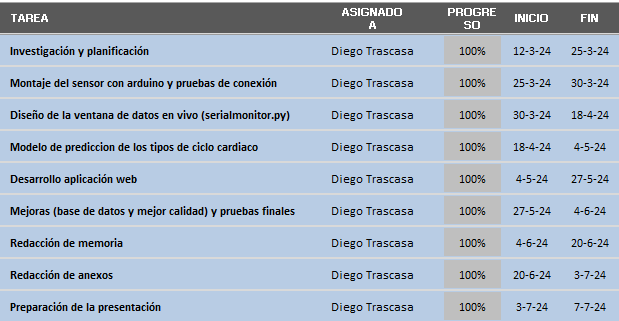
\includegraphics[width=1\textwidth]{img/gantt.png}
\caption{Diagrama de Gantt final}
\label{fig:gantt}
\end{figure}

\section{Planificación económica}

Cuando se planea un proyecto, es fundamental tener en cuenta todos los gastos, incluyendo el software, los materiales y los salarios. También es crucial considerar las posibles formas de obtener ingresos con el proyecto.

Esta sección presenta el cálculo del presupuesto del proyecto, cubriendo desde el desarrollo de la página web hasta las mejoras realizadas en un prototipo de hardware.

\subsection{Coste de personal}

Este proyecto ha sido realizado por un solo individuo, desde la concepción hasta la implementación. Se considerará como un Ingeniero Biomédico (equivalente a Ingeniería de la Salud) . En España, el salario promedio para un Ingeniero Biomédico recién graduado es de aproximadamente 27.000 €/año \cite{infojobs}. Para un proyecto de 3 meses de duración, el coste del empleado sería de aproximadamente 6.750 €. Además, se debe considerar el costo de la Seguridad Social, que según el Régimen General de la Seguridad Social \cite{seguridadsocial}, puede calcularse con porcentajes específicos aplicados al salario bruto, Tabla \ref{tab:costesEmpleado}.

\begin{table}[h]
\centering
\begin{tabular}{ll}
\hline
\rowcolor[HTML]{FFFFFF} \textbf{Sueldo bruto al mes } & 2.250 €\\ \hline
\rowcolor[HTML]{EFEFEF} \multicolumn{2}{|c|}{\textbf{Costes Seguridad Social}} \\ \hline
\rowcolor[HTML]{FFFFFF} Contingencias Comunes (23,60\%) & 531 €\\ \hline
\rowcolor[HTML]{EFEFEF} Contrato (6,7\%) & 150,75 €\\ \hline
\rowcolor[HTML]{FFFFFF} Fondo de Garantía Salarial (0,2\%) & 4,50 \\ \hline
\rowcolor[HTML]{EFEFEF} Formación Profesional (0,6\%) & 13,50 €\\ \hline
\rowcolor[HTML]{FFFFFF} \textbf{Costo total - 1 mes} & \textbf{2.949,75 €} \\ \hline
\rowcolor[HTML]{C0C0C0} \textbf{Costo total - 2 meses} & \textbf{5.899,50 €} \\ \hline
\rowcolor[HTML]{FFFFFF} \textbf{Costo total - 3 meses} & \textbf{8.849,75 €} \\ \hline
\end{tabular}
\caption{Costes de contratación}
\label{tab:costesEmpleado}
\end{table}

\subsection{Costes de software}

Las herramientas utilizadas en el proyecto son Anaconda, Streamlit, y Arduino IDE, todas ellas son de código abierto y gratuitas.

\subsection{Amortización de los equipos}

El equipo principal y unico que se ha utilizado ha sido un portátil HP, con un precio de compra aproximado de 550 € y una vida estimada de 5 años. La amortización durante los tres meses que ha durado el proyecto se calcula con la siguiente fórmula:

\[
\text{Amortización} = \frac{\text{Precio}}{\text{Vida Útil(Años)}} \times \frac{\text{Meses Usado}}{12}
\]

Aplicando esta fórmula, se obtiene una amortización de 27,5 €, como podemos ver en la Tabla \ref{table:amortizacion} \cite{financialtimes}.

\begin{table}[h]
\centering
\begin{tabular}{|l|r|}
\hline
\rowcolor[HTML]{EFEFEF} \textbf{Concepto} & \textbf{Valor} \\
\hline Precio de Compra & 550 € \\
\hline Vida Útil & 5 años \\
\hline Meses de Uso & 3 meses \\
\hline Amortización del Periodo & 27,5 € \\
\hline
\end{tabular}
\caption{Cálculo de la amortización del portátil HP}
\label{table:amortizacion}
\end{table}




\subsection{Costes de hardware}

Para estimar el precio del prototipo utilizado en las pruebas del proyecto, se realizó una comparación de precios de los componentes necesarios en tiendas online como Amazon, Mouser Electronics y SparkFun. Se decidió optar por Amazon y Mouser Electronics debido a su fiabilidad y disponibilidad de productos.

A continuación, se presenta una tabla con los componentes utilizados y sus respectivos costos (Tabla \ref{tabla-costes-hardware}):

\begin{table}[h]
    \centering
    \begin{tabular}{ll}
        \hline
        \rowcolor[HTML]{FFFFFF} 
        \textbf{Componente} & \textbf{Coste (€)} \\ \hline
        \rowcolor[HTML]{EFEFEF} 
        Arduino UNO R3 & 24,00 \\ \hline
        \rowcolor[HTML]{FFFFFF} 
        Cables & 1,50 \\ \hline
        \rowcolor[HTML]{EFEFEF} 
        Electrodos & 12,00 \\ \hline
        \rowcolor[HTML]{FFFFFF} 
        Módulo AD8232 & 14,00 \\ \hline
        \rowcolor[HTML]{EFEFEF} 
        Caja 3D & 3,00 \\ \hline
        \rowcolor[HTML]{FFFFFF} 
        LED & 1,20 \\ \hline
        \rowcolor[HTML]{EFEFEF} 
        Resistencias & 0,80 \\ \hline
        \rowcolor[HTML]{C0C0C0} 
        \textbf{Coste Total} & \textbf{56,50 €} \\ \hline
    \end{tabular}
    \caption{Desglose de costes de los componentes del prototipo.}
    \label{tabla-costes-hardware}
\end{table}


El presupuesto se basó en precios disponibles en Amazon \cite{amazon} y Mouser Electronics \cite{mouser}. Aunque se evaluaron otras opciones como AliExpress, se descartaron debido a problemas de confiabilidad y tiempos de entrega.



\section{Viabilidad legal}

La viabilidad legal del proyecto es crucial para asegurar la protección de los datos y el cumplimiento de las normativas vigentes. A continuación, se detallan las leyes y normativas aplicables:

\subsection{Protección de datos personales}

Para garantizar la privacidad y seguridad de la información hay que cumplir con las normas de protección de datos ya que se esta trabajando con datos sensibles con lo son los ECG.

\begin{itemize}
    \item \textbf{Reglamento (UE) 2016/679 (RGPD)}:  Este reglamento establece las normas para el tratamiento y libre circulación de datos personales en la Unión Europea, garantizando derechos como el acceso, rectificación y eliminación de los datos por parte de los usuarios \cite{boe_rgpd}.
    \item \textbf{LOPDGDD 3/2018}: Esta ley complementa el RGPD en España, regulando aspectos específicos del tratamiento de datos en el ámbito digital \cite{boe_lopd}.
    \item \textbf{Ley 41/2002, básica reguladora de la autonomía del paciente y de derechos y obligaciones en materia de información y documentación clínica}: Protege los derechos y la confidencialidad de datos de los pacientes \cite{boe_paciente}.
\end{itemize}

\subsection{Comercialización de Dispositivos Médicos}

Para garantizar la seguridad, eficacia y calidad del dispositivo desarrollado, se deben cumplir las siguientes normativas:

\begin{itemize}
    \item \textbf{Reglamento (UE) 2017/745 sobre los productos sanitarios}: Regula la seguridad y comercialización de los productos sanitarios dentro de la UE, incluyendo software de seguimiento médico \cite{boe_productos_sanitarios}.
    \item \textbf{Marcado CE (Conformidad Europea)}: Indica que el dispositivo cumple con los requisitos de seguridad y protección establecidos por la UE, permitiendo su libre circulación dentro del mercado europeo \cite{boe_ce}.
    \item \textbf{Real Decreto 192/2023 por el que se regulan los productos sanitarios}: Define la clasificación y regulación de productos sanitarios en España, siendo responsabilidad de la Agencia Española de Medicamentos y Productos Sanitarios \cite{boe_rd}.
\end{itemize}

\subsection{Derechos de autor y propiedad intelectual}

El software desarrollado, así como cualquier contenido original, debe estar protegido por las leyes de derechos de autor y propiedad intelectual:

\begin{itemize}
    \item \textbf{Directiva (UE) 2009/24/CE sobre la protección jurídica de programas de ordenador}: Protege los programas de ordenador como obras originales, aplicando derechos de autor \cite{boe_software}.
    \item \textbf{Real Decreto Legislativo 1/1996 por el que se aprueba el texto refundido de la Ley de Propiedad Intelectual}: Establece las bases de la propiedad intelectual y los derechos de autor en España \cite{boe_propiedad_intelectual}.
\end{itemize}
